\documentclass[a4paper,11pt]{article}
\usepackage[T1]{fontenc}
\usepackage[utf8]{inputenc}
\usepackage{lmodern}
\usepackage{amssymb}
\usepackage{amsmath}
\usepackage[swedish,english]{babel}
\usepackage{epsfig}
%\usepackage[usenames,dvipsnames]{pstricks}
%\usepackage{svg}
\title{Fysik}
\author{Jakob Tigerström/Eric Johansson}

\begin{document}
\maketitle
\tableofcontents
\newpage
\begin{flushleft}
\section{TODO}
\begin{itemize}
  \item Fyll på SI-Systemet
  \item Skriv fler föreläsningar
  \item Strukturera upp föreläsningarna med section/subsection
  \item Lägg in uppgifts pappren.
  \item Skriv snyggare i allmänhet.
  \item Skriv mer om massa enhet.
\end{itemize}
\section{Prefix}

\begin{tabular}{l c r}
  Femto & f & $ 10^{-15} $\\ 
  Piko & p & $ 10^{-12} $\\ 
  Nano & n & $ 10^{-9} $\\ 
  Mickro & $ \mu $ & $ 10^{-6} $\\ 
  Milli & m & $ 0,001 = 10^{-3} $\\
  Centi & c & $ 0,01 = 10^{-2} $\\
  Deci & d & $ 0,1 = 10^{-1}$\\
  Deka & da & $ 10 = 10^1 $\\
  Hekto & h & $ 100 = 10^2 $\\
  Kilo & k & $ 1000 = 10^3 $\\
  Mega & M & $ 10^6 $\\
  Giga & G & $ 10^9 $\\
  Tera & T & $ 10^{12} $\\
  Peta & P & $ 10^{15} $\\
  Exa & E & $ 10^{18} $\\
  Zetta & Z & $ 10^{21} $\\
  Yotta & Y & $ 10^{24} $\\
\end{tabular}
\newpage
\section{SI-Systemet}
SI-Systemet är en internationell standard för måttenheter och prefix. SI-Systemet består av 7 storheter som har en enhet som är noggrant definierad. 
Det finns även ett antal herledda enheter från SI-Systemet.\newline
SI-Systemet består av följande storheter:
\begin{itemize}
  \item längd (l,s)
  \item massa (m)
  \item tid (t)
  \item elektrisk ström (I)
  \item temperatur (K)
  \item ljusstyrka (I)
  \item substandsmängd (n)
\end{itemize}

\subsection{Längd ($l,s$)- meter (m)}
Från början var en metern definerad av distansen mellan Nordpolen och ekvatorn so man bestämde var $ 10^7 $ meter.
Man gjorde kopior på metern som kallas arkivmetern.
1 meter är den sträcka som ljuset rör sig i vakum på $ \frac{1}{299792458} $ sekund.
\newline
\newline
\subsection{Massa ($m$)- kilogram (kg)}
Från en början (år 1793) var måttenheten för massa grave och definitionen var 1$dm^3$ vid 0$^{\circ}$C är 1 grave.
Dock ansångs det att grave var för stor enhet att mäta i och då skapades gramme vilket är en tusendel av 1 grave.
Men dem insåg att gramme var för liten enhet att mäta i så dem återvände till grave, dock kunde det inte heta grave. 
Utan fick namnet kilogramme, 1000 gramme, och är den enda enheten i SI-Systemet med ett prefix.\newline\newline
År 1799 definerades kilogram till att 1 liter vatten vid 4$^{\circ}$C har massan 1kg. 4$^{\circ}$C är den temperaturen
då vattnet är som "kompakt"/densitet.\newline
Sedan skapades en ren platinum-cylinder med samma vikt som definitionen för massa och placerades ut i arkiv runt om i värlen.\newline\newline
År 1889 uppgraderades cylindern till en platinum-iridium-mixad cylinder med samma massa och placerades ut i arkiv runt om i värlen.\newline\newline
År 1948 så samlades alla cylindrar för att vägas och det visade sig att massan hade ändrats med tiden.\newline\newline
År 1992 vägdes samltiga cylindrar igen och massan hade fortsatt sin förändring.\newline\newline
Massan är den enda enheten i SI-Systemet som har en fysisk definition, för tillfället.\newline
\textit{Man håller på att göra en sfär av matriallet silikon-28 med massan 1kg. När den är skapad så kommer man
ränka ut antalet silikon-28 atomer vilket kommer bilda den nya definitionen av massa. https://www.youtube.com/watch?v=ZMByI4s-D-Y}
\newline
\newline
\subsection{Tid ($t$)- Sekunder (s)}
Idag är definitionen att 1 sekund är varaktigheten av 9 192 631 770 perioder av den strålning som motsvarar övergången mellan de två 
hyperfinnivåerna i grundtillståndet hos atomen cesium-133 (atomur). \newline \newline
Ursprungligen var sekunden $ \frac{1}{24*60*60} $ del av medelsoldygnet.
\newline

\subsection{Elektrisk ström ($I$) - ampere (A)}
1 ampere är storleken av den konstanta elektriska ström som, då den genomflyter två parallella, raka ledare med oändlig längd och försumbard cirkulärt tvärsnitt och placeade på ett avstånd från varandra av 1 meter i vakuum, mellan dessa ledare åstakommer en kraft lika med 2$*$10$^{-7}$ newton per meter av ledarens längd.

\subsection{Temperatur ($T$) - Kelvin (K)}
1 Kelvin är bråkdelen $\frac{1}{273,16}$ av den termodynamiska temperaturan vid vattnets trippelpunkt.

\subsection{Ljusstyrka ($I$) - candela (cd)}
1 candela är ljusstyrkan i en given rikning hos en monokromatisk strålning vars frekvens är 540$*$10$^{12}$ hertz vars strålningsstyrka i denna rikning är $\frac{1}{683}$ watt per steradian.

\subsection{Substandsmängd ($n$) - mol (mol)}
1 mol är substansmängden i ett system innehållande lika mångs systemelement som det finns atomer i 0,012kilogram kol-12. Antalet är Avogadros tal 6,022$*$10$^{23}$ per mol.

\subsection{Härledda enheter}
Nedan listast några av de härledda enheterna som används mycket inom fysik.
\begin{tabular}{llll}
Storhet & Härledd enhet & Beteckning & Samband med grundenhet \\\hline
Area, $A$ & 1 kvadratmeter & 1m$^2$ & 1m$^2$ \\\hline
Densitet, $\rho$ & 1kg per kubikmeter & 1kg/m$^3$ & 1kg/m$^3$ = 1kg $*$ m$^{-3}$ \\\hline
Hastighet, $v$ & 1 meter per sekund & 1 m/s & 1m/s = 1 m $*$ s$^{-1}$ \\ \hline
Acceleration, $a$& 1 meter per sekundtvå & 1m/s$^2$ & 1m/s$^2$ = 1 m $*$ s$^{-2}$ \\ \hline
Volym, $v$ & 1 kubikmeter & 1 m$^3 $ & 1 m$^3 $ \\ \hline
Kraft $F$ & 1 newton & 1N & 1N = 1 kg $*$ m $*$ $s^{-2}$
\end{tabular}
\newpage
\section{Ränkte exempel}
Nedan listast några räkne exempel som tagits upp på lektionstid och använder SI-Systemet och de härledda enheterna.

\subsection{Beräkna area på oljefläck} Vid en olje tanks rensning spreds 340 $ dm^3 $ olja ut på ett tunnt skikt på vattenytan.
Oljeskiktet var 2.5nm tjockt.\newline
Hur stor area hade oljebältet.\newline

\begin{tabular}{l l | c r}
  Storhet & Beteckning & Enhet & Beteckning\\
  Längd & l & meter & m\\
  Massa & m & kilogram & kg\\
  Tid & t & sekund & s\\
\end{tabular}

\subsection{Massa/volym}

\begin{tabular}{l c r}
  Massa(g) & Volym i mätglaset(ml) & Stenarnas volym(ml)\\
  0 & 62 & 0\\
  16.6 & 68 & 6\\
  29.9 & 73 & 11\\
  46.2 & 79 & 17\\
  62.9 & 85 & 23\\
  73.3 & 88 & 26\\
\end{tabular}
\newline
\newline
$ m = \rho * V  $
\newline
$ \rho = \frac{m}{V} $
\newline
$ \rho = 2.714285714 = \frac{76}{28} $\newline
$ \rho = 2,7 g/ml = \frac{2,6 g}{1 ml} = \frac{2,6 g}{0,001 dm} $
\newpage

\subsection{Densitet på en kula/sfär}
En kula med radien 12,5 mm har massan 61g.\newline
Bestäm kulans densitet.\newline
$ m = 61g = 0,061 kg $\newline
$ V = \frac{4\pi r^3}{3} = \frac{4\pi 0,0125^3}{3} \approx 8,181230869*10^{-6} m^3 $\newline
$ \rho = \frac{m}{V} = \frac{0,061}{8,181230869*10^{-6}} \approx 7,5*10^3 kg/m^3 $\newline
\newline
\subsection{Thomaskorv}
Hur mycket korv kan man göra av Thomas?\newline
$ V = A*l $\newline
Thomas volym?\newline
Thomas massa: $ m=110kg $\newline
$ V \rho = \frac{mV}{\rho} $\newline
$ \frac{V\rho}{\rho} = \frac{m}{\rho} $\newline
$ V = \frac{m}{\rho} $ \newline
Thomas densitet $ \approx $ vattnets densitet.\newline
$ \rho = 0,998 g/cm^3 = 998 kg/m^3 $\newline
$ V= \frac{m}{\rho} = 0,11 m^3 $\newline
$ r = 1,5 cm $ Thomas korv\newline
$ A = r^2 \pi = (0,015)^2 =\approx 7,068*10^-4 $\newline
$ \rho = \frac{V}{A} = \frac{0,11}{7,068*10^-4} $\newline
\newline
\subsection{Uppskata luftens massa i en sal}
Uppskatta massan för luften i föreläsnings salen.\newline
$ \rho = \frac{m V}{V} $\newline
$ m = \rho V = 1293 * 540 \approx 700 kg $\newline
$ \rho = 1,293 kg/m^3 $\newline
$ V = 12 * 15 * 3  \approx 540 m^3 $
Mätnoggranhet\newline
Anger närmevärdet med felgränsen\newline
$ A = 0,305 m^2 $\newline
$ 0,3045 \leqslant  A \leqslant  0,3055 m^3 $ 3 gällande siffror\newline
\newpage
\section{Viktig regel}
Om du gör en multiplikation eller division ska svaret innehålla så många gällande siffror som det minst noggranna ingångs värde\newline\newline
Om du gör en addition eller subtraktion ska svaret ha lika många decimaler som det ingångsvärde som har minst antal decimaler.
\newline
\subsection{EX1}
En matta har längden(\textit{l}) 12,71 m och bredden(\textit{b}) 3,46 m.\newline
Vilken area har mattan?\newline
$ A = lb = 12,71 * 3,46 \approx 43,9766 m^2 \approx 44,0 m^2 $\newline

\section{Övningar}
\subsection{Densitet}
Koppar folie massa: $m=13g=0,013kg $\newline
Koppar folie densitet: $ \rho=\frac{m}{V} $ $ V=\frac{m}{\rho} = \frac{0,013}{8,96*10^3} $\newline
$ h=\frac{V}{A}=1,45*10^{-6} $
\subsection{Mätning}
$ t=\frac{13min}{2}=6,5min $
$ v= 0,300*10^4 m/s $\newline
$ v=\frac{s}{t} $\newline
$ s=v*t = (0,300*10^9)*(6,5*60)=1,2*10^{11}m $
\section{Repetition}
\subsection{Tyngd(tyngdkraft)}
$ F=m*g $\newline
$ g=9,82 N/kg $\newline
Tyngdkraft är gravitationskraft vid jordytan.\newline
$ G=6,673*10^{-11}\frac{Nm^2}{kg^2} $
\subsubsection{Newtons allmänna gravitationslag}
$ F=G\frac{m_1 m_2}{r^2} $
\subsubsection{EX1}
$ F=G\frac{m_1 m_2}{r^2}=6,673*10^{-11} $\newline
$ F=G(\frac{90*100}{0,85^2})=8,3*10^{-7}N $\newline
\subsubsection{EX2}
Jordradien är 637 mil. Upskatta jordens massa.\newline
$ F=G\frac{m_{Tomas} m_{Jorden}}{r^2}=m_{Tomas}*g $\newline
$ m_{Jorden}=\frac{gr^2}{G}=\frac{9,28*6370000}{6,673*10^{-11}}=6,0*10^{24} $
\subsection{Normalkraft}
Normalkraft = $F_N=$\newline
Normal betyder \textit{vinkelrät mot.}\newline
I detta fall är normalkraften lika stor som tyngdkraften.
\subsection{Spännkraft(linkraft)}
\subsection{Friktionskraft}
Friktionskraft $( F_f )$\newline
\newpage
\section{Uppgifter}
\subsection{Rörelse 3}
\begin{enumerate}
  \item \begin{enumerate}
    \item $ s=11,3cm=0,113m $\newline
    $ t=0,07s $\newline
    $ \frac{0,113m}{0,07s}=1,6m/s $\newline
    Svar: Medel hastigheten är $ 1,6m/s $.
    \item Vet ej.
  \end{enumerate}
  \item $ 42,67+60=102,67s $\newline
  $ \frac{800}{102.67}=7,79m/s $\newline
  \newline
  $ \frac{102,67}{3600}=0,0285 = 102,67s $ i timmar$(h)$\newline
  \newline
  $ \frac{0,8}{0,0285}=28,07km/h\approx28,0km/h $\newline
  \newline
  Svar: Han färdas $ 7,79m/s $ eller $ 28,0km/h $  
  
  \item $ 3600s/h $\newline
  $ 86400s/d $\newline
  $ 86400*3,3nm/s=285120nm/d $\newline
  $ 0,285mm/d $\newline
  $ \frac{20mm}{0,285}=70 $\newline
  Svar: Det tar 70 dygn tills håret är $2cm$ längre.
  \item \begin{enumerate}
    \item $ V_m=\frac{21}{13,2}=1,6m/s $\newline
    \item $ V_m=\frac{21*2}{13,2+8,5}=\frac{42}{21,7}=1,935\approx1,9m/s $\newline
  \end{enumerate}
  \item $ V_m=\frac{35}{30}=1,2m/s $
  \item \begin{enumerate}
    \item Fråga6
  \end{enumerate}
\end{enumerate}
\newpage
\subsection{Uppgift 34 i Fysik}
$ t_{gå}=50s $\newline
$ t_{rull}=75s $\newline
$ t_{total}=?$\newline
$ V_{gå}=\frac{s}{t_{gå}}=\frac{s}{50} $\newline
$ V_{rull}=\frac{s}{t_{rull}}=\frac{s}{75} $\newline
$ V_{tot}=V_{gå}+V_{rull} $\newline
$ V_{tot}=\frac{3s}{150}+\frac{2s}{150}=\frac{5s}{150} $\newline
$ s=V_{tot}*t_{tot} $\newline
$ t_{tot}=\frac{s}{V_{tot}} $\newline
$ t_{tot}=\frac{s}{\frac{5s}{150}}=s/\frac{5s}{150}=\frac{s}{1}*\frac{150}{5s}=30 $\newline
Svar: $30s$
\section{EX1}
Lådan har massan $m$ kg.
Rita ut krafterna på lådan om den ligger stilla.\newline
Tyngden = mg\newline
$ F_N  \neq $ mg
\section{EX2}
Metallkulan har tyngden 3,2N. Magneten attraherar metall kulan med kraftern $ 5,1N $. Rita in normalkraften i figuren och beräkna normalkraftens sorlek. Metallkulans tyngdkraft är $ 3,9N $.\newline
$ F_N+3,2=5,1 $\newline
$ F_N=5,1-3,1=1,9N $
\section{Newtons Lagar}
\subsection{Tröghetslagen} Att en kropp inte påverkas av någon resulterande kraft är ekvivalent med att den behåller sitt rörelsetillstånd.\newline
$ F_{res}<=> \Delta v=0 $
\newline
\subsection{Kraftlagen}
Om ett föremål med massan, m, påverkas av en resulterande kraft, $ F_{res} $ så kommer föremålet att accelerera med acceleration ,a. $ F_{res}=ma $
\subsection{Lagen om verkan och motverkan}
Om en kropp A påverkar en kropp B med en kraft, så påverkar B kroppen A med en lika stor men motsatt riktad kraft.
\subsubsection{EX1}
En bil med massan $880kg$ accelererar från 0 till $108km/h$ på $9,0s$.\newline
Beräkna den resulterande kraft som krävs för detta.\newline
$ a=\frac{\Delta v}{\Delta t}=\frac{(108-0)/3,6}{9,0}=3,3m/s^2 $\newline
$ F_{res}=ma=880*3,3=2933,33\approx1900N=2,9kN $
\subsection{EX1}
En fallskärms hoppare väger med utrustning $62kg$ efter att falskärmen utvecklats får hon den konstanta farten $20km/h$.\newline
Vilka krafter verkar på henne?\newline
$F_{luftmotstånd} $
$ Tyngd=62*gN \approx 609N $
\section{Lutande plan}
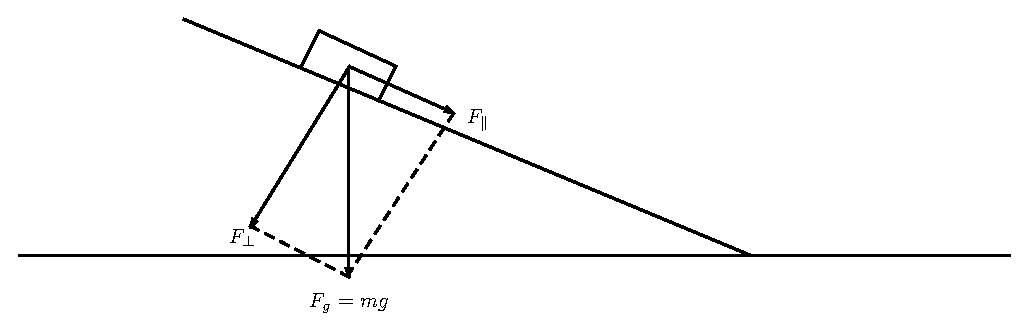
\includegraphics{lutandeplan.eps}\newline
$ F_g = mg = 2,0*9,82 = 19,64 N $\newline
$ \sin v = \frac{F_{\parallel}}{F_g} $\newline
$ 19,64 \sin 25 = \frac{F_{\parallel}}{19,64} = 8,3 N $\newline\newline
Svar: $ F_{\parallel} \approx 8,3N $
\section{Newtons andra lag}
$ F_{res} = ma $
\subsection{EX1}
Vi släpper en blomkruka från andra vångingen. Den har massan $2,0kg$
Hur stor blir accelerationen om vi har en luftmotståndskraft $ F_L = 0,5 N $\newline
$ F_{res} = 19,64 - 0,5 = 19,14 N $\newline
$ F_{res} = ma = 2,0a $\newline
$ 2,0a = 19,14 $\newline
$ a = \frac{19,14}{2,0} \approx 9,6 m/s^2 $
\subsection{EX2}
En gris har massan $8,0 kg$, vill inte följa med på promenaden. Bestäm accelerationen om friktionskoefficienten är 0,6 mot underlaget.\newline
$ F = 50N $\newline
$ F_F = \mu F_N = \mu mg = 0,6*8,0*9,82 \approx 47,136 $\newline
$ F_{res} = 50-47,136 \approx 2,864 N $
$ F_{res} = ma = 8,0a $\newline
$ 8,0a = 1,864 $\newline
$ a = \frac{2,864}{8} \approx 0,36m/s^2 $
\subsection{EX3}
En helikopter lyfter en ren med massan $150kg$ med en konstant hastighet uppåtriktad på $2,0m/s$\newline
\begin{enumerate}
  \item Bestäm kraften i repen\newline
  $ F_g = mg = 150*9,82 = 1473N $\newline
  $ F_{rep} = F_g = 1473N \approx 1500N$\newline
  \item $ F_g = mg = 1473N $\newline
  $ F_{res} = ma = 150*2,0 = 300N $\newline
  $ F_{res} = F_{rep}-F_g = F_{rep}-1473 $\newline
  $ F_{rep} = 1773N \approx 1800N $\newline  
\end{enumerate}
\section{Trigonometri}
\subsection{Exempel på nästan allt}
Ett föremål med massan $5,3kg$ befinner sig på ett lutande plan där friktionstalet mellan föremål och plan är $0,30$.\newline
Vilken acceleration får föremålet?\newline
Tyngdkraften: $mg = 5,4*9,82 = 52N$\newline
$ \cos 25 = \frac{F_{\perp}}{52} $\newline
$ F_{\perp} = 52 * \cos 25 = 47,2 N $\newline
$ \sin 25 = \frac{F_{\parallel}}{52} $\newline
$ F_{\parallel} 52*sin 25 = 22,0 N $\newline

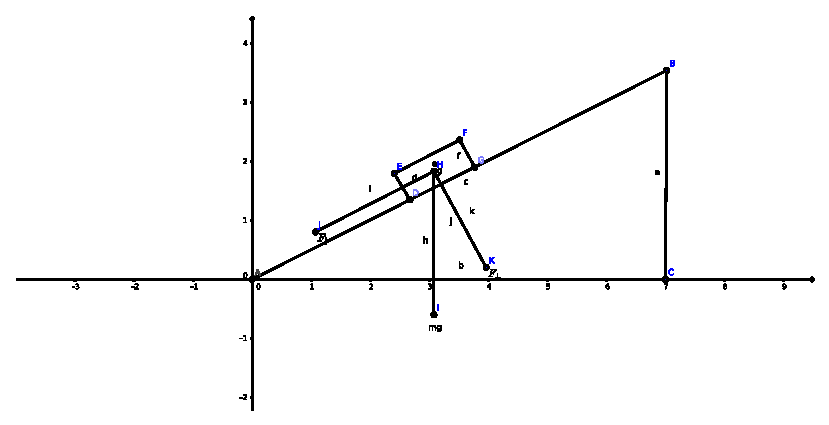
\includegraphics{trigonometri.eps}\newline
Friktionskraften:\newline
$ F_f = \mu * F_N = 0,30 * 47,2 = 14,2 N $\newline
Resultanten: $ F_{\parallel} - F_f $\newline
$ 22,0 - 14,2 = 7,8 N $\newline
$ F_{res} = ma $\newline
$ a = \frac{F_{res}}{m} = \frac{7,8}{5,3} = 1,5 m/s^2 $\newline
\section{Rörelselagar}
Konstant acceleration\newline
$ a = konstant $\newline

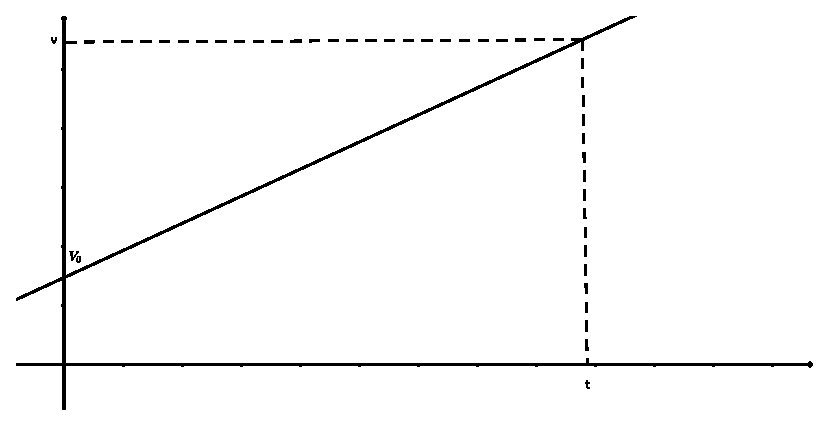
\includegraphics{vt_diagram.eps}\newline
$ a = \frac{\Delta v}{\Delta t} $\newline
$ a*t = \frac{v-v_0}{t}*t $\newline
$ at = v-v_0 $\newline
$ v = v_0tat $\newline
Förflyttningen ges av arean under grafen.\newline
$ S = v_0 t+\frac{(v+v_0)*t}{2} = v_0 t +\frac{vt-v_0t}{2} = v_0t+\frac{vt}{2}-\frac{v_0t}{2} $\newline
$ \frac{v_0t+vt}{2} = \frac{(v_0+v)t}{2} $\newline
$ S = \frac{v_0t+vt}{2} = \frac{v_0t+(v0+at)t}{s} = \frac{v_0t+v_0t+at^2}{2} = \frac{2v_0t+at^2}{2} = v_0t+\frac{at^2}{2} $\newline\newline
$ a = \frac{v-v_0}{t} * \frac{S}{S} = \frac{v-v_0}{t} * \frac{\frac{(v_0+v)t}{2}}{s} = \frac{v-v_0t}{2} = \frac{1}{S} $\newline
$ a2s = (v-v_0)(v+v_0) = v^2-v_0^2 $\newline
\subsection{EX1}
Från en bro, 15 m över vattnet släpps en sten. Använd $g\approx 10m/s^2$
\begin{enumerate}
  \item När kommer stenen ner?\newline
  $ v_0 = 0$\newline
  $ a = g $\newline
  $ S = v_0t+\frac{at^2}{2} $\newline
  $ 15 = 0*t+\frac{10t^2}{2} $\newline
  $ 15 = 5t^2 $\newline
  $ t^2 = \frac{15}{5} = 3 $\newline
  $ t = \sqrt{3} \approx 1,7s $
  \item Vilken fart har den då?
  $ v = v_0 + at = 0+10*1,7 = 17 m/s $
  \subsection{EX2}
  En annan sten kastas från bron med hastigheten 100 m/s rakt uppåt. Använd $g\approx 10m/s^2$
  \begin{enumerate}
    \item När kommer stenen ner?\newline
      $ a = g $\newline
      $ v_0 = -10,0 m/s $\newline
      $ S = v_0t+\frac{at^2}{2} $\newline
      $ 15 = -10t+\frac{10t^2}{2} $\newline
      $ 15 = -10t+5t^2 $\newline
      $ 0 = 5t^2-10t-15 $\newline
      $ \frac{5t^2-10t-15}{5} $\newline
      $ 0 = t^2-2t-3 $\newline
      $ t = 1 \pm \sqrt{1^2-(-3)} $\newline 
      $ t = 1 \pm \sqrt{4} = t = 1 \pm 2 $\newline 
      $ t = 1 $ eller $ t = 3 $\newline
    \item Vilken fart har den då?
    $ v = v_0+at $\newline
    $ v = -10+10*3 $\newline
    $ v = 20 m/s $
  \end{enumerate}
\end{enumerate}
\end{flushleft}
\end{document}
